\section{Filters}\label{sec:filters}
Filters are needed to cancel out noise from the acceleration inputs.
Noise is caused by electronic noise from the circuitry and mechanical noise from the sensor itself \citep{misc:SensorsMag}.

\subsection{The Kalman Filter} 
%The theory from this section is based on \citet{electronic:KalmanGreg}.
The Kalman filter is built upon a simple found propagation in a dynamic Bayesian network, where the previous state and new observations is used to find the current state.
A Bayesian network can be used to find the probability distribution of the next state given the current state.
The Kalman filter is a linear dynamic system, which means the function derived will be a linear function.

The Kalman filter structure can be modelled as a dynamic Bayesian network, see \figref{fig:kalman-filter}.
Insertion of evidence in the network will be described in \secref{section:insert-evidence}.
Additional theory for Kalman filters exists, but has not been examined, as it was unnecessary for this project.
\begin{figure}[H]
	\centering
	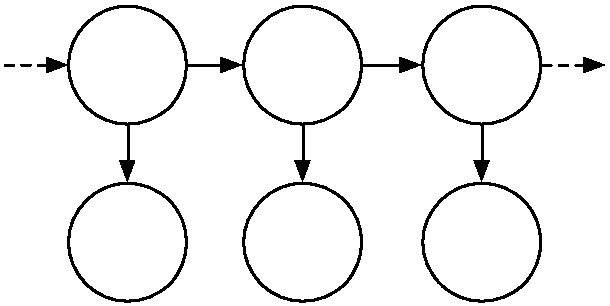
\includegraphics[scale=0.6]{media/kalman-filter}
	\caption{The Kalman filter.}
	\label{fig:kalman-filter}
\end{figure}

\begin{comment}
The state equation is:
\begin{equation*}
	 \textbf{x}_{k} = \textbf{F}_{k} \textbf{x}_{k-1} + \textbf{B}_{k} \textbf{u}_{k-1} + \textbf{W}_{k-1}
\end{equation*}
where
\begin{itemize}
	\item[$x_k$] is a state matrix at state $k$.
	\item[$F_k$] is the state transition matrix that is applied to the previous state matrix $x_{k-1}$.
	\item[$B_k$] is the transition matrix from the previous state $u_{k-1}$.
	\item[$W_k$] is the noise gained from the previous states, also called Guassian noise.
\end{itemize}


The previous state can also include noise, because of uncertainty of the measurement, and thus do not have an accurate value, this must therefore be taken into account.
To find the previous state measurement value, a linear function combining the sensor value and the measurement noise is used.
\end{comment}

\subsection{Exponential Moving Average}
\label{subsection:exponential-moving-average}
The exponential moving average (EMA) reduces noise from the input and smoothes the data set.
The formula for exponential moving average is as follows:
\begin{equation*}
	EMA_i = \alpha * y_i + (1-\alpha) * EMA_{i-1}
\end{equation*}
where,
\begin{itemize}
	\item[]
	\begin{itemize}
		\item[$EMA_i$] is the exponential moving average value for the i'th data element.
		\item[$\alpha$] is a coefficient which determines the smoothness of the data.
		\item[$y_i$] is the i'th observed value.
	\end{itemize}
\end{itemize}
$EMA_i$ is calculated recursively, updating the values. 
The previously observed values are accounted for in the formula by $EMA_{i-1}$ but their impact is reduced in each step.
The formula works by weighing the new value and adding it with the weighted previously observed values $EMA_{i-1}$.
\figref{fig:EMA} shows two graphs where the red graph is the raw data and green is the data after running the exponential moving average, with an $\alpha$ of $0.1$.

\begin{figure}[H]
	\centering
	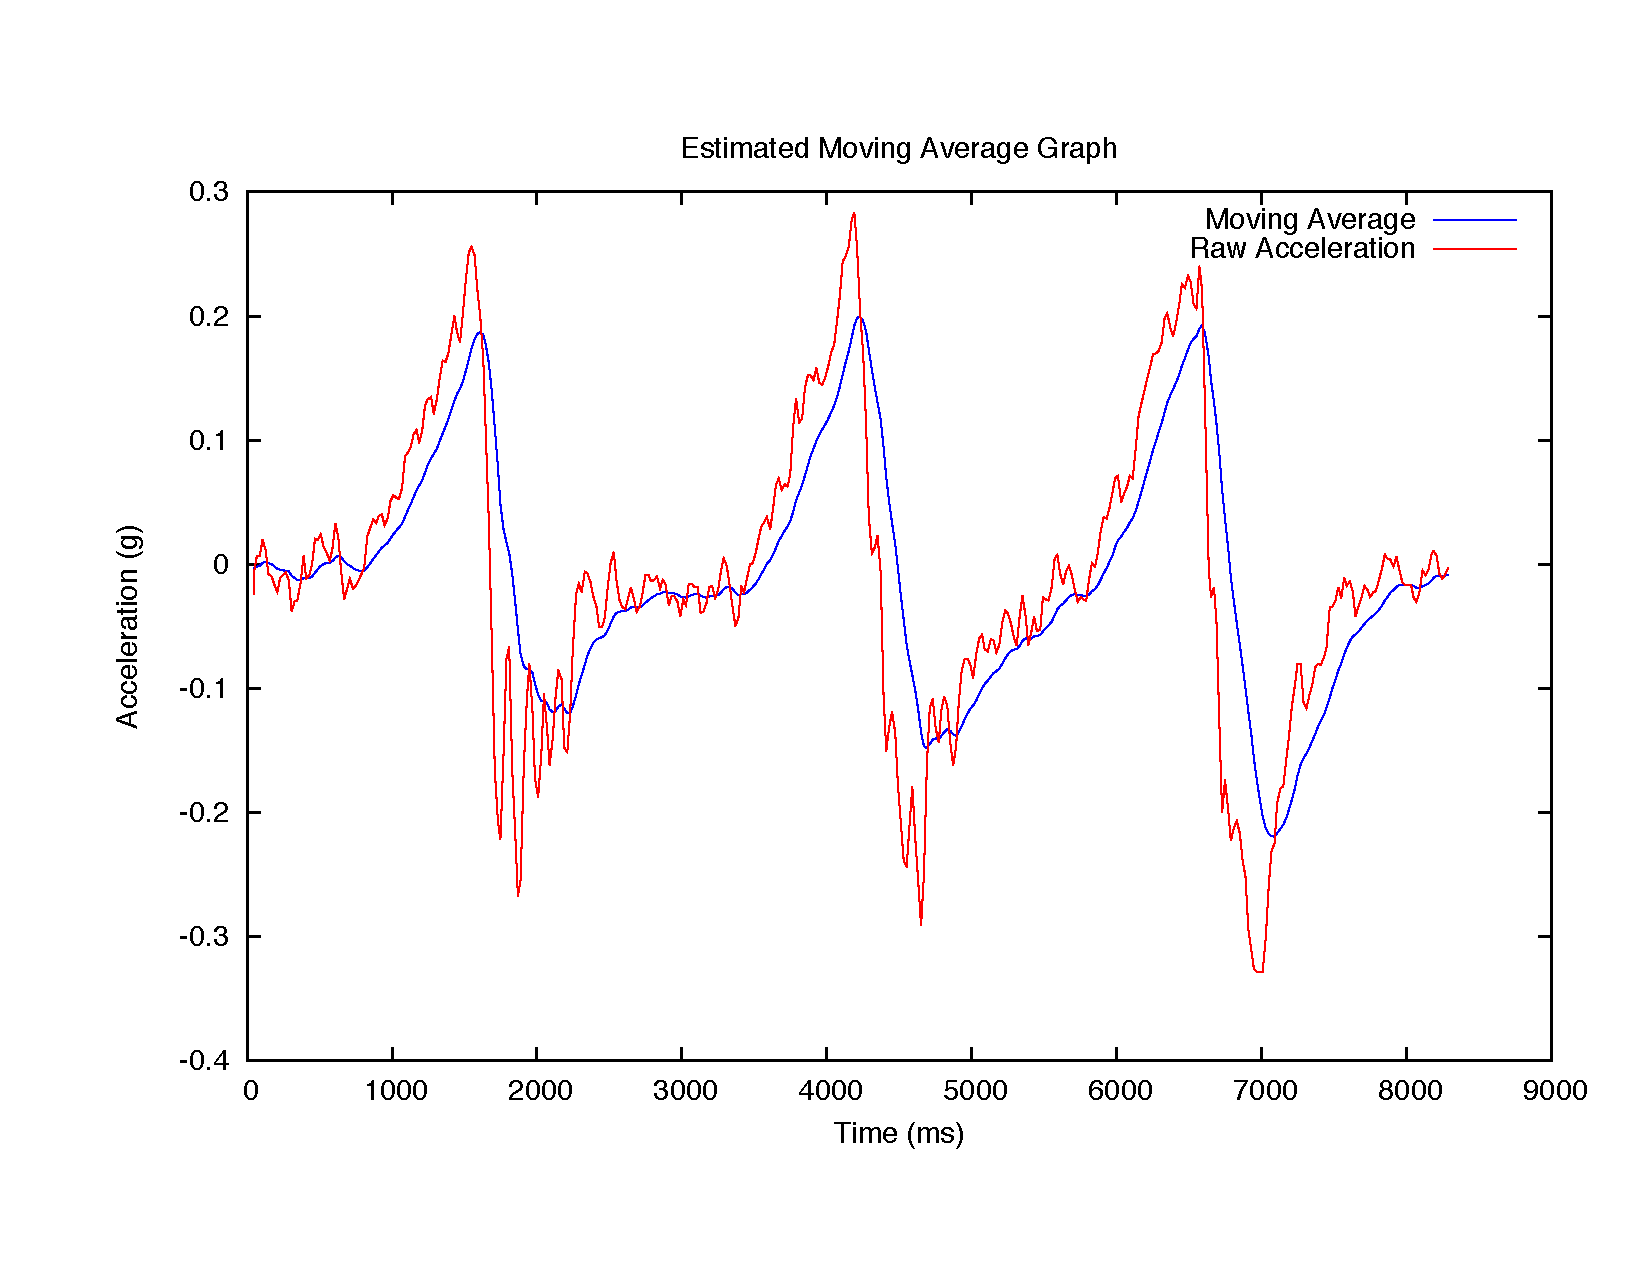
\includegraphics[scale=0.45, trim=0cm 2cm 0cm 2cm]{media/gnuplot/ema.pdf}
	\caption{Raw data, red graph, compared with the EMA data, blue graph.}
	\label{fig:EMA}
\end{figure}
